\documentclass[a3paper,xelatex,english]{bxjsarticle}
\usepackage{pgfplots,pgfplotstable}
\pgfplotsset{ compat = newest }
\usepackage{tikz}
\usetikzlibrary{arrows.meta,bending,calc,shapes,positioning}
\usepackage{ascmac}
\usepackage{fancybox}
\usepackage{amsmath,amssymb}
\usepackage{algorithm}
\usepackage[edges]{forest}
\usepackage{array}
\usepackage{algpseudocode}
\usepackage{paralist}
\usepackage{cases}
\usepackage{fvextra}
\usepackage{colortbl}
\usepackage{xcolor}
\usepackage{fancyhdr}
\usepackage[explicit]{titlesec}
\usepackage{xspace}
\usepackage[many]{tcolorbox}
\usepackage{lastpage}
\usepackage{verbatim}
\usepackage{multirow}
\usepackage{censor}
\usepackage[unicode,pdftitle={Report of Entropy estimates based on NIST SP 800-90B non-IID track},setpagesize=false]{hyperref}
\usepackage[open,openlevel=4]{bookmark}
\newcommand\mib[1]{\boldsymbol{#1}}
\usepgfplotslibrary{patchplots}
%%%%%%%%%%%%%%%%%%%%%%%%%%%%%%%%%%%%%%%%%%%%%%%%%%%%%%%%%%%%%%%%%%%%%%%%%%%%%%%
%%%%%%
%%%%%% customize page numbering
%%%%%%
%%%%%%%%%%%%%%%%%%%%%%%%%%%%%%%%%%%%%%%%%%%%%%%%%%%%%%%%%%%%%%%%%%%%%%%%%%%%%%%
\fancypagestyle{mypagestylewithtotalpagenumbers}{
\lhead{}
\rhead{}
\cfoot{\thepage/\pageref{LastPage}}
\renewcommand{\headrulewidth}{0.0pt}
}
%%%%%%%%%%%%%%%%%%%%%%%%%%%%%%%%%%%%%%%%%%%%%%%%%%%%%%%%%%%%%%%%%%%%%%%%%%%%%%%
%%%%%%
%%%%%% output up to 4-th level
%%%%%%
%%%%%%%%%%%%%%%%%%%%%%%%%%%%%%%%%%%%%%%%%%%%%%%%%%%%%%%%%%%%%%%%%%%%%%%%%%%%%%%
\setcounter{secnumdepth}{4}
\setcounter{tocdepth}{4}
\setlength{\topmargin}{-1cm}
\setlength{\textheight}{37cm}
%%%%%%%%%%%%%%%%%%%%%%%%%%%%%%%%%%%%%%%%%%%%%%%%%%%%%%%%%%%%%%%%%%%%%%%%%%%%%%%
%%%%%%
%%%%%%
%%%%%%
%%%%%%%%%%%%%%%%%%%%%%%%%%%%%%%%%%%%%%%%%%%%%%%%%%%%%%%%%%%%%%%%%%%%%%%%%%%%%%%
%%%\renewcommand{ \figurename }{Figure }
%%%\renewcommand{ \tablename }{Table }
%%%\renewcommand{ \refname }{References}
%%%%%%%%%%%%%%%%%%%%%%%%%%%%%%%%%%%%%%%%%%%%%%%%%%%%%%%%%%%%%%%%%%%%%%%%%%%%%%%
%%%%%%
%%%%%%
%%%%%%
%%%%%%%%%%%%%%%%%%%%%%%%%%%%%%%%%%%%%%%%%%%%%%%%%%%%%%%%%%%%%%%%%%%%%%%%%%%%%%%
\definecolor{rowcolorlightblue}{RGB}{191,233,251}
\definecolor{bordercolordarkblue}{RGB}{0,163,243}
\definecolor{BleuDur}{RGB}{27,61,176}
\definecolor{Nigelle}{RGB}{0,133,201}
\definecolor{BleuFaience}{RGB}{105,171,219}
\definecolor{anotherlightblue}{RGB}{61,143,244}
%%%%%%%%%%%%%%%%%%%%%%%%%%%%%%%%%%%%%%%%%%%%%%%%%%%%%%%%%%%%%%%%%%%%%%%%%%%%%%%
%%%%%%
%%%%%%
%%%%%%
%%%%%%%%%%%%%%%%%%%%%%%%%%%%%%%%%%%%%%%%%%%%%%%%%%%%%%%%%%%%%%%%%%%%%%%%%%%%%%%
\def\chpcolor{BleuDur}
\def\chpcolortxt{BleuDur}
\def\sectionfont{\sffamily\LARGE}
%%%%%%%%%%%%%%%%%%%%%%%%%%%%%%%%%%%%%%%%%%%%%%%%%%%%%%%%%%%%%%%%%%%%%%%%%%%%%%%
%%%%%%
%%%%%%
%%%%%%
%%%%%%%%%%%%%%%%%%%%%%%%%%%%%%%%%%%%%%%%%%%%%%%%%%%%%%%%%%%%%%%%%%%%%%%%%%%%%%%
\makeatletter
%Section:
\def\@sectionstrut{\vrule\@width\z@\@height12.5\p@}
\def\@makesectionhead#1{%
  {\par\vspace{20pt}%
   \parindent 0pt\raggedleft\sectionfont
   \colorbox{\chpcolor}{%
     \parbox[t]{90pt}{\color{white}\@sectionstrut\@depth4.5\p@\hfill
       \ifnum\c@secnumdepth>\z@\thesection\fi}%
   }%
   \begin{minipage}[t]{\dimexpr\textwidth-90pt-2\fboxsep\relax}
   \color{\chpcolortxt}\@sectionstrut\hspace{5pt}#1
   \end{minipage}\par
   \vspace{10pt}%
  }
}
\def\section{\@afterindentfalse\secdef\@section\@ssection}
\def\@section[#1]#2{%
  \ifnum\c@secnumdepth>\m@ne
    \refstepcounter{section}%
    \addcontentsline{toc}{section}{\protect\numberline{\thesection}#1}%
  \else
    \phantomsection
    \addcontentsline{toc}{section}{#1}%
  \fi
  \sectionmark{#1}%
  \if@twocolumn
    \@topnewpage[\@makesectionhead{#2}]%
  \else
    \@makesectionhead{#2}\@afterheading
  \fi
}
\def\@ssection#1{%
  \if@twocolumn
    \@topnewpage[\@makesectionhead{#1}]%
  \else
    \@makesectionhead{#1}\@afterheading
  \fi
}
\makeatother
%%%%%%%%%%%%%%%%%%%%%%%%%%%%%%%%%%%%%%%%%%%%%%%%%%%%%%%%%%%%%%%%%%%%%%%%%%%%%%%
%%%%%%
%%%%%%
%%%%%%
%%%%%%%%%%%%%%%%%%%%%%%%%%%%%%%%%%%%%%%%%%%%%%%%%%%%%%%%%%%%%%%%%%%%%%%%%%%%%%%
\setlength{ \topmargin }{-1.5cm}
%%%%%%%%%%%%%%%%%%%%%%%%%%%%%%%%%%%%%%%%%%%%%%%%%%%%%%%%%%%%%%%%%%%%%%%%%%%%%%%
%%%%%%
%%%%%%
%%%%%%
%%%%%%%%%%%%%%%%%%%%%%%%%%%%%%%%%%%%%%%%%%%%%%%%%%%%%%%%%%%%%%%%%%%%%%%%%%%%%%%
\pagestyle{mypagestylewithtotalpagenumbers}
%%%%%%
%%%%%%
%%%%%%
\title{Report of Entropy estimates based on NIST SP 800-90B non-IID track}
\date{2023-Nov-04 08:13:07.622863}
\begin{document}
%\StopCensoring
\maketitle
%%%%%%%%%%%%%%%%%%%%%%%%%%%%%%%%%%%%%%%%%%%%%%%%%%%%%%%%%%%%%%%%%%%%%%%%%%%%%%%
%%%%%%
%%%%%%%%%%%%%%%%%%%%%%%%%%%%%%%%%%%%%%%%%%%%%%%%%%%%%%%%%%%%%%%%%%%%%%%%%%%%%%%
\thispagestyle{mypagestylewithtotalpagenumbers}
%%%%%%%%%%%%%%%%%%%%%%%%%%%%%%%%%%%%%%%%%%%%%%%%%%%%%%%%%%%%%%%%%%%%%%%%%%%%%%%
%%%%%%
%%%%%%%%%%%%%%%%%%%%%%%%%%%%%%%%%%%%%%%%%%%%%%%%%%%%%%%%%%%%%%%%%%%%%%%%%%%%%%%
\section{Identification information}
\subsection{Identification of acquisition data from entropy source}
\renewcommand{\arraystretch}{1.8}
\begin{table}[h]
\caption{Identification information of acquisition data from entropy source}
\begin{center}
\begin{tabular}{|>{\columncolor{anotherlightblue}}p{2cm}|p{20.5cm}|}
\hline 
URL of the acquisition data & \url{https://github.com/usnistgov/SP800-90B_EntropyAssessment/blob/master/bin/rand4_short.bin} \\
\hline
SHA-256 hash value of the acquisition data [hex] & 
\begin{verbatim}
a9e2169c b1accc78 cd23892d 793a232b 84b0cd13 ccc39235 26e0b207 62bd77ac
\end{verbatim} 
\\
\hline
\end{tabular}
\end{center}
\end{table}
\renewcommand{\arraystretch}{1.8}
\begin{itemize}
		\item Name of the submitter of the acquisition data : 
		    \begin{Form}
		    \noindent
		    \TextField[name=NameOfSubmitter, multiline=false, bordercolor=bordercolordarkblue,width=12cm]{}
		    \end{Form}
		\item Brief explanation of the acquisition data (or entropy source) : \\
		    \begin{Form}
		    \noindent
		    \TextField[name=ExplanationOfAcquisitionData, multiline=true, bordercolor=bordercolordarkblue,width=\linewidth,height=1in]{}
		    \end{Form}
	\end{itemize} 
\subsection{Identification of analysis environment}
\renewcommand{\arraystretch}{1.8}
\begin{table}[h]
\caption{Identification information of analysis environment}
\begin{center}
\begin{tabular}{|>{\columncolor{anotherlightblue}}l|>{\columncolor{anotherlightblue}}l|p{12cm}|}
\hline 
Analysis tool & Name & Another entropy estimation tool with extensions \\
\cline{2-3}
\, & Versioning information & 1.0.50 \\
\cline{2-3}
\, & built as &  64-bit application \\
\cline{2-3}
\, & built by &  Intel C++ Compiler ( \verb|__INTEL_LLVM_COMPILER|: 20230202 ) \\
\cline{2-3}
\, & linked libraries &  Boost C++ 1.83.0 \\
\hline
Analysis environment & Hostname & \censor{PANTHERF340} \\
\cline{2-3}
\, & CPU information & Intel(R) Core(TM) i5\censor{-10500T CPU @ 2.30GHz} \\
\cline{2-3}
\, &  Physical memory size & \censor{65239} MiB \\
\cline{2-3}
\, &  OS information & Windows 10 or greater 64-bit \\
\cline{2-3}
\, &  Username & \censor{genya} \\
\hline
\end{tabular}
\end{center}
\end{table}
\renewcommand{\arraystretch}{1.4}
\subsection{Identification of analysis conditions}
\renewcommand{\arraystretch}{1.8}
\begin{table}[h]
\caption{Identification information of analysis conditions}
\begin{center}
\begin{tabular}{|>{\columncolor{anotherlightblue}}l|p{8cm}|}
\hline 
Number of samples & 10000 \\
\hline
Bits per sample & 4 \\
\hline
Byte to bit conversion & 
Most Significant bit (MSb) first
 \\
\hline
\end{tabular}
\end{center}
\end{table}
\renewcommand{\arraystretch}{1.4}
\subsection{Identification of analysis method}
NIST SP 800-90B \cite{SP80090B} 6.3 with corrections \cite{CorrectionsSP80090B} is applied
\clearpage
\section{Executive summary}
\subsection{Numerical results of min-entropy estimates based on non-IID track}
\pgfplotstableread{
section	y	y-min	y-max
6.3.1	 3.79004	0.00208717	       0
6.3.5	 3.56747	       0	       0
6.3.6	 3.83353	       0	       0
6.3.7	 3.86695	0.00221569	0.0022192
6.3.8	 3.78365	0.00207483	0.0020779
6.3.9	 3.88466	0.00222981	0.00223336
6.3.10	  3.8825	0.0022298	0.00223335
}{\summarytableNonBinary}
\pgfplotstableread{
section	y	y-min	y-max
6.3.1	0.979189	7.1102e-05	       0
6.3.2	 0.89818	0.00339469	0.00352477
6.3.3	0.990617	0.000142204	       0
6.3.4	0.803872	       0	       0
6.3.5	0.898777	       0	       0
6.3.6	0.932969	       0	       0
6.3.7	0.986561	7.15801e-05	7.15837e-05
6.3.8	0.982642	7.12728e-05	7.12763e-05
6.3.9	0.977697	7.10275e-05	7.1031e-05
6.3.10	0.980145	7.11764e-05	7.11799e-05
}{\summarytableBinary}
\begin{table}[h]
\caption{Numerical results}
\begin{center}
\begin{tabular}{|l|c|c|c|c|}
\hline 
\rowcolor{anotherlightblue} %%
Estimator										& $H_{\textrm{original}}$$^{\textrm{\,a}}$			& Notes to $H_{\textrm{original}}$  & $H_{\textrm{bitstring}}$$^{\textrm{\,b}}$	& Notes to $H_{\textrm{bitstring}}$			\\ 
\cline{2-5}
\rowcolor{anotherlightblue} %%
\,												& [bit / 4 - bit] & \, & [bit / 1 - bit] &	\,	\\
\hline 
The Most Common Value Estimate					& 3.79004& see \ref{sec:NonBinary631} & 0.979189& see \ref{sec:Binary631} \\
\hline 
The Collision Estimate							& ---		  & --- & 0.89818& see \ref{sec:Binary632} \\
\hline 
The Markov Estimate								& ---		  & --- & 0.990617& see \ref{sec:Binary633} \\
\hline 
The Compression Estimate						& ---		  & --- & 0.803872& see \ref{sec:Binary634} \\
\hline 
The t-Tuple Estimate							& 3.56747& see \ref{sec:NonBinary635} & 0.898777& see \ref{sec:Binary635} \\
\hline 
The Longest Repeated Substring (LRS) Estimate	& 3.83353& see \ref{sec:NonBinary636} & 0.932969& see \ref{sec:Binary636} \\
\hline 
Multi Most Common in Window Prediction Estimate	& 3.86695& see \ref{sec:NonBinary637} & 0.986561& see \ref{sec:Binary637} \\
\hline 
The Lag Prediction Estimate						& 3.78365& see \ref{sec:NonBinary638} & 0.982642& see \ref{sec:Binary638} \\
\hline 
The MultiMMC Prediction Estimate				& 3.88466& see \ref{sec:NonBinary639} & 0.977697& see \ref{sec:Binary639} \\
\hline 
The LZ78Y Prediction Estimate					& 3.8825& see \ref{sec:NonBinary6310} &0.980145& see \ref{sec:Binary6310} \\
\hline \hline 
The intial entropy source estimate [bit / 4 - bit]	& \multicolumn{4}{|c|}{3.21549}	\\
$H_{I} = \min (H_{\textrm{original}}, 4\times H_{\textrm{bitstring}})$ &\multicolumn{4}{ | c | } {\, }	\\
\hline \hline 
\multicolumn{5}{|l|}{$^{\,a}$\quad Entropy estimate of the sequential dataset [source: NIST SP 800-90B \cite{SP80090B} 3.1.3]} \\
\multicolumn{5}{|l|}{$^{\,b}$\quad An additional entropy estimation (per bit) for the non-binary sequential dataset [see NIST SP 800-90B \cite{SP80090B} 3.1.3]} \\
\hline 
\end{tabular}
\end{center}
\end{table}
\clearpage
\subsection{Visual comparison of min-entropy estimates from original samples}
\begin{figure}[htbp]
\centering

\begin{tikzpicture} 
\begin{axis}
	[symbolic x coords={6.3.1,6.3.2,6.3.3,6.3.4,6.3.5,6.3.6,6.3.7,6.3.8,6.3.9,6.3.10},
	width=18cm,
	ymin=0,
	ymax=4,
	xlabel=Sub-sub-section of NIST SP 800-90B,
	ylabel={Estimated min-entropy $[$bit / 4-bit$]$},
	xtick=data]
\addplot+[forget plot,only marks] 
  plot[error bars/.cd, y dir=both, y explicit]
  table[x=section,y=y,y error plus expr=\thisrow{y-max},y error minus expr=\thisrow{y-min}] {\summarytableNonBinary};
\addplot+[Nigelle,no marks,sharp plot,update limits=false] 
coordinates {(6.3.1,3.56747) (6.3.10,3.56747)}
node[below] at (axis cs:6.3.5,3.56747) {Estimated min-entropy = 
3.56747};
\end{axis} 
\end{tikzpicture}

\caption{Estimated Min-Entropy using $\S$6.3 of NIST SP 800-90B}
\end{figure}
\subsection{Visual comparison of min-entropy estimates by interpreting each sample as bitstring}
\begin{figure}[htbp]
\centering

\begin{tikzpicture} 
\begin{axis}
	[symbolic x coords={6.3.1,6.3.2,6.3.3,6.3.4,6.3.5,6.3.6,6.3.7,6.3.8,6.3.9,6.3.10},
	width=18cm,
	ymin=0,
	ymax=1,
	xlabel=Sub-sub-section of NIST SP 800-90B,
	ylabel={Estimated min-entropy $[$bit / 1-bit$]$},
	xtick=data]
\addplot+[forget plot,only marks] 
  plot[error bars/.cd, y dir=both, y explicit]
  table[x=section,y=y,y error plus expr=\thisrow{y-max},y error minus expr=\thisrow{y-min}] {\summarytableBinary};
\addplot+[Nigelle,no marks,sharp plot,update limits=false] 
coordinates {(6.3.1,0.803872) (6.3.10,0.803872)}
node[below] at (axis cs:6.3.5,0.803872) {Estimated min-entropy = 
0.803872};
\end{axis} 
\end{tikzpicture}

\caption{Estimated Min-Entropy using $\S$6.3 of NIST SP 800-90B}
\end{figure}
\clearpage
\section{Detailed results of analysis from original samples}
\subsection{The Most Common Value Estimate (NIST SP 800-90B Section 6.3.1)}\label{sec:NonBinary631}

\begin{figure}[htbp]
\centering

\begin{tikzpicture}
\begin{axis}[
	ybar,
	bar width=1.25pt,
	xmin=-0.125,
xmax=15.125,	ymin=0,
	width=20cm,
	xlabel=$x_i$,
	ylabel=\#$\{x_i \,\textrm{in} \,S\} / L$
]
\addplot coordinates {
(       0,   0.0585)
(       1,   0.0637)
(       2,   0.0626)
(       3,   0.0635)
(       4,   0.0653)
(       5,   0.0629)
(       6,   0.0631)
(       7,   0.0576)
(       8,   0.0659)
(       9,   0.0602)
(      10,   0.0605)
(      11,   0.0634)
(      12,   0.0638)
(      13,   0.0627)
(      14,   0.0651)
(      15,   0.0612)
};
\addplot+[Nigelle,no marks,sharp plot,update limits=false] 
coordinates {(0,0.0659) (15,0.0659)}
node[above] at (axis cs:7.5,0.0659) {\shortstack{$\hat{p}$ = 
0.0659\\($\rightarrow$ min-entropy = 3.79004 [bit / 4-bit])}};
\end{axis}
\end{tikzpicture}

\caption{Distribution of $x_i$}
\end{figure}
\subsubsection{Supplemental information for traceability}
\renewcommand{\arraystretch}{1.8}
\begin{table}[h]
\caption{Supplemental information for traceability (NIST SP 800-90B Section 6.3.1)}
\begin{center}
\begin{tabular}{|l|c|}
\hline 
\rowcolor{anotherlightblue} %%
Symbol				& Value \\ \hline 
mode				&      659\\ \hline 
$\hat{p}$ 			&   0.0659\\ \hline
$p_u$				& 0.0722911\\ \hline
\end{tabular}
\end{center}
\end{table}
\renewcommand{\arraystretch}{1.4}
\clearpage
\subsection{The t-tuple Estimate (NIST SP 800-90B Section 6.3.5)}\label{sec:NonBinary635}

\begin{figure}[htbp]
\centering

\begin{tikzpicture}
\begin{semilogyaxis}[
	width=20cm,
	xlabel=$i$,
	ylabel=$Q \lbrack i \rbrack $
]
\addplot coordinates {
(   1, 659)
(   2, 60)
};
\end{semilogyaxis}
\end{tikzpicture}

\caption{Intermediate value $Q[i]$ \, in $\S$6.3.5 of NIST SP 800-90B}
\end{figure}
\begin{figure}[htbp]
\centering

\begin{tikzpicture}
\begin{axis}[
	width=20cm,
	xlabel=$i$,
	ylabel=$\left( P \lbrack i \rbrack \right)^{1/i}$,
	/pgf/number format/.cd,fixed,precision=6
]
\addplot coordinates {
(   1,   0.0659)
(   2, 0.0774635)
};
\addplot+[Nigelle,no marks,sharp plot,update limits=false] 
coordinates {(1,0.0774635) (2,0.0774635)}
node[above left] at (axis cs:2,0.0774635) {\shortstack{$\hat{p}_{\textrm{max}}$ = 0.0774635\\($\rightarrow$ min-entropy = 3.56747 [bit / 4-bit])}};
\end{axis}
\end{tikzpicture}

\caption{$P[i]^{1/i}$ \, in $\S$6.3.5 of NIST SP 800-90B}
\end{figure}
\clearpage
\subsubsection{Supplemental information for traceability}
\renewcommand{\arraystretch}{1.8}
\begin{table}[h]
\caption{Supplemental information for traceability (NIST SP 800-90B Section 6.3.5)}
\begin{center}
\begin{tabular}{|l|c|}
\hline 
\rowcolor{anotherlightblue} %%
Symbol				& Value \\ \hline 
$t$				&        2\\ \hline 
$\hat{p}_{\textrm{max}}$ 			& 0.0774635\\ \hline
$p_u$				& 0.0843497\\ \hline
\end{tabular}
\end{center}
\end{table}
\renewcommand{\arraystretch}{1.4}
\clearpage
\subsection{The LRS Estimate (NIST SP 800-90B Section 6.3.6)}\label{sec:NonBinary636}

\begin{figure}[htbp]
\centering

\begin{tikzpicture}
\begin{axis}[
	view/h=160,
	colormap/bluered, colorbar horizontal,
	width=20cm,
	ymin=2,
	xlabel=$W$,
	ylabel=$C_i$,
	zlabel=multiplicity,
]
\addplot3[surf, mesh/ordering=y varies, shader=faceted interp] coordinates {
(   3,   2,    1054)  (   3,   3,     903)  (   3,   4,     527)  (   3,   5,     240)  (   3,   6,      99)  (   3,   7,      34)  (   3,   8,      12)  (   3,   9,       2)  (   3,  10,       5)  

(   4,   2,     661)  (   4,   3,      30)  (   4,   4,       2)  (   4,   5,       0)  (   4,   6,       0)  (   4,   7,       0)  (   4,   8,       0)  (   4,   9,       0)  (   4,  10,       0)  

(   5,   2,      53)  (   5,   3,       0)  (   5,   4,       0)  (   5,   5,       0)  (   5,   6,       0)  (   5,   7,       0)  (   5,   8,       0)  (   5,   9,       0)  (   5,  10,       0)  

(   6,   2,       3)  (   6,   3,       0)  (   6,   4,       0)  (   6,   5,       0)  (   6,   6,       0)  (   6,   7,       0)  (   6,   8,       0)  (   6,   9,       0)  (   6,  10,       0)  

};
\end{axis}
\end{tikzpicture}

\caption{Estimated $W$-tuple collision probability in Step 3 of $\S6.3.6$ of NIST SP 800-90B}
\end{figure}
\begin{figure}[htbp]
\centering

\begin{tikzpicture}
\begin{axis}[
	width=20cm,
	xlabel=$W$,
	ylabel=$\left( P_W \right) ^{i/W}$,
    ticklabel style={
        % change "directory" to the number format
        /pgf/number format/.cd,
            fixed,
        % change "directory" back to tikz
        /tikz/.cd,
    },
	yticklabel style = { /pgf/number format/precision=6 }
]
\addplot  coordinates {
(   3, 0.0624249)
(   4, 0.0625122)
(   5, 0.0638468)
(   6, 0.0625804)
};
\addplot+[Nigelle,no marks,sharp plot,update limits=false] 
coordinates {(3,0.0638468) (6,0.0638468)}
node[above, xshift=-10mm] at (axis cs:5,0.0638468) {\shortstack{$\hat{p}$ = 0.0638468 \\($\rightarrow$ min-entropy = 3.83353 [bit / 4-bit])}};
\end{axis}
\end{tikzpicture}

\caption{Estimated average collision probability per string symbol in Step 3 of $\S6.3.6$ of NIST SP 800-90B}
\end{figure}
\clearpage
\subsubsection{Supplemental information for traceability}
\renewcommand{\arraystretch}{1.8}
\begin{table}[h]
\caption{Supplemental information for traceability (NIST SP 800-90B Section 6.3.6)}
\begin{center}
\begin{tabular}{|l|c|}
\hline 
\rowcolor{anotherlightblue} %%
Symbol				& Value \\ \hline 
$u$				&        3\\ \hline 
$v$				&        6\\ \hline 
$\hat{p}$ 			& 0.0638468\\ \hline
$p_u$				& 0.0701445\\ \hline
\end{tabular}
\end{center}
\end{table}
\renewcommand{\arraystretch}{1.4}
\clearpage
\subsection{Multi Most Common in Window Prediction Estimate (NIST SP 800-90B Section 6.3.7)}\label{sec:NonBinary637}

\begin{figure}[htbp]
\centering

\begin{tikzpicture}
\begin{axis}[
	ybar,
	xmin=0,
	ymin=0,
	width=20cm,
	xlabel=length of run of ones in $correct$,
	ylabel=occurences
]
\addplot+[ybar] coordinates {
(       1,       2)
(       2,       1)
};
\addplot+[Nigelle,no marks,sharp plot,update limits=false] 
coordinates {(2, 1) (2, 1)}
node[above left] at (axis cs:2, 1) {\shortstack{$r - 1$ = 2 
\\($\rightarrow$ min-entropy = 3.86695 [bit / 4-bit])}};
\end{axis}
\end{tikzpicture}
\caption{Distribution of $correct$}
\end{figure}
\subsubsection{Supplemental information for traceability}
\renewcommand{\arraystretch}{1.8}
\begin{table}[h]
\caption{Supplemental information for traceability (NIST SP 800-90B Section 6.3.7)}
\begin{center}
\begin{tabular}{|l|c|}
\hline 
\rowcolor{anotherlightblue} %%
Symbol				& Value \\ \hline 
$N$				& 9937\\ \hline 
$C$				& 619\\ \hline 
$P_{\textrm{global}}$				& 0.0622924\\ \hline 
$P'_{\textrm{global}}$			& 0.0685379\\ \hline 
$r$				& 3\\ \hline 
$P_{\textrm{local}}$ 			& 0.0100725\\ \hline
\end{tabular}
\end{center}
\end{table}
\renewcommand{\arraystretch}{1.4}
\clearpage
\subsection{Lag Prediction Estimate (NIST SP 800-90B Section 6.3.8)}\label{sec:NonBinary638}

\begin{figure}[htbp]
\centering

\begin{tikzpicture}
\begin{axis}[
	ybar,
	xmin=0,
	ymin=0,
	width=20cm,
	xlabel=length of run of ones in $correct$,
	ylabel=occurences
]
\addplot+[ybar] coordinates {
(       1,       2)
(       2,       1)
(       3,       1)
};
\addplot+[Nigelle,no marks,sharp plot,update limits=false] 
coordinates {(3, 1) (3, 1)}
node[above left] at (axis cs:3, 1) {\shortstack{$r - 1$ = 3 
\\($\rightarrow$ min-entropy = 3.78365 [bit / 4-bit])}};
\end{axis}
\end{tikzpicture}
\caption{Distribution of $correct$}
\end{figure}
\subsubsection{Supplemental information for traceability}
\renewcommand{\arraystretch}{1.8}
\begin{table}[h]
\caption{Supplemental information for traceability (NIST SP 800-90B Section 6.3.8)}
\begin{center}
\begin{tabular}{|l|c|}
\hline 
\rowcolor{anotherlightblue} %%
Symbol				& Value \\ \hline 
$N$				& 9999\\ \hline 
$C$				& 662\\ \hline 
$P_{\textrm{global}}$				& 0.0662066\\ \hline 
$P'_{\textrm{global}}$			& 0.0726119\\ \hline 
$r$				& 4\\ \hline 
$P_{\textrm{local}}$ 			& 0.0319235\\ \hline
\end{tabular}
\end{center}
\end{table}
\renewcommand{\arraystretch}{1.4}
\clearpage
\subsection{The MultiMMC Prediction Estimate (NIST SP 800-90B Section 6.3.9)}\label{sec:NonBinary639}

\begin{figure}[htbp]
\centering

\begin{tikzpicture}
\begin{axis}[
	ybar,
	xmin=0,
	ymin=0,
	width=20cm,
	xlabel=length of run of ones in $correct$,
	ylabel=occurences
]
\addplot+[ybar] coordinates {
(       1,       2)
(       2,       1)
(       3,       1)
};
\addplot+[Nigelle,no marks,sharp plot,update limits=false] 
coordinates {(3, 1) (3, 1) }
node[above left] at (axis cs:3, 1) {\shortstack{$r - 1$ = 3 
\\($\rightarrow$ min-entropy = 3.88466 [bit / 4-bit])}};
\end{axis}
\end{tikzpicture}
\caption{Distribution of $correct$}
\end{figure}
\subsubsection{Supplemental information for traceability}
\renewcommand{\arraystretch}{1.8}
\begin{table}[h]
\caption{Supplemental information for traceability (NIST SP 800-90B Section 6.3.9)}
\begin{center}
\begin{tabular}{|l|c|}
\hline 
\rowcolor{anotherlightblue} %%
Symbol				& Value \\ \hline 
$N$				& 9998\\ \hline 
$C$				& 615\\ \hline 
$P_{\textrm{global}}$				& 0.0615123\\ \hline 
$P'_{\textrm{global}}$			& 0.0677021\\ \hline 
$r$				& 4\\ \hline 
$P_{\textrm{local}}$ 			& 0.0319243\\ \hline
\end{tabular}
\end{center}
\end{table}
\renewcommand{\arraystretch}{1.4}
\clearpage
\subsection{The LZ78Y Prediction Estimate (NIST SP 800-90B Section 6.3.10)}\label{sec:NonBinary6310}

\begin{figure}[htbp]
\centering

\begin{tikzpicture}
\begin{axis}[
	ybar,
	xmin=0,
	ymin=0,
	width=20cm,
	xlabel=length of run of ones in $correct$,
	ylabel=occurences
]
\addplot+[ybar] coordinates {
(       1,       2)
(       2,       1)
(       3,       1)
};
\addplot+[Nigelle,no marks,sharp plot,update limits=false] 
coordinates {(3, 1) (3, 1)}
node[above left] at (axis cs:3, 1){\shortstack{$r - 1$ = 3 
\\($\rightarrow$ min-entropy = 3.8825 [bit / 4-bit])}};
\end{axis}
\end{tikzpicture}
\caption{Distribution of $correct$}
\end{figure}
\subsubsection{Supplemental information for traceability}
\renewcommand{\arraystretch}{1.8}
\begin{table}[h]
\caption{Supplemental information for traceability (NIST SP 800-90B Section 6.3.10)}
\begin{center}
\begin{tabular}{|l|c|}
\hline 
\rowcolor{anotherlightblue} %%
Symbol				& Value \\ \hline 
$N$				& 9983\\ \hline 
$C$				& 615\\ \hline 
$P_{\textrm{global}}$				& 0.0616047\\ \hline 
$P'_{\textrm{global}}$			& 0.0678035\\ \hline 
$r$				& 4\\ \hline 
$P_{\textrm{local}}$ 			& 0.0319364\\ \hline
\end{tabular}
\end{center}
\end{table}
\renewcommand{\arraystretch}{1.4}
\clearpage
\section{Detailed results of analysis by interpreting each sample as bitstrings}
\subsection{The Most Common Value Estimate (NIST SP 800-90B Section 6.3.1)}\label{sec:Binary631}

\begin{figure}[htbp]
\centering

\begin{tikzpicture}
\begin{axis}[
	ybar,
	bar width=5pt,
	xmin=-0.125,
xmax=1.125,	ymin=0,
	width=20cm,
	xlabel=$x_i$,
	ylabel=\#$\{x_i \,\textrm{in} \,S\} / L$
]
\addplot coordinates {
(       0, 0.500825)
(       1, 0.499175)
};
\addplot+[Nigelle,no marks,sharp plot,update limits=false] 
coordinates {(0,0.500825) (1,0.500825)}
node[above] at (axis cs:0.5,0.500825) {\shortstack{$\hat{p}$ = 
0.500825\\($\rightarrow$ min-entropy = 0.979189 [bit / 1-bit])}};
\end{axis}
\end{tikzpicture}

\caption{Distribution of $x_i$}
\end{figure}
\subsubsection{Supplemental information for traceability}
\renewcommand{\arraystretch}{1.8}
\begin{table}[h]
\caption{Supplemental information for traceability (NIST SP 800-90B Section 6.3.1)}
\begin{center}
\begin{tabular}{|l|c|}
\hline 
\rowcolor{anotherlightblue} %%
Symbol				& Value \\ \hline 
mode				&    20033\\ \hline 
$\hat{p}$ 			& 0.500825\\ \hline
$p_u$				& 0.507265\\ \hline
\end{tabular}
\end{center}
\end{table}
\renewcommand{\arraystretch}{1.4}
\clearpage
\subsection{The Collision Estimate (NIST SP 800-90B Section 6.3.2)}\label{sec:Binary632}

\begin{figure}[htbp]
\centering

\begin{tikzpicture}
\begin{axis}[
	ybar,
	xmin=0,
	xtick={0, 1, 2, 3},
	ymin=0,
	width=20cm,
	xlabel=$t_{\nu}$,
	ylabel=occurences of $t_{\nu}$
]
\addplot+[ybar] coordinates {
(       2,     7856)
(       3,     8096)
};
\addplot+[Nigelle,no marks,sharp plot,update limits=false] 
coordinates {(2.49733,8096) (2.49733,1)}
node[above right] at (axis cs:2.49733,8096) {$\bar{X}'$ = 2.49733};
\end{axis}
\end{tikzpicture}

\caption{Distribution of intermediate value $t_{\nu}$}
\end{figure}
\begin{figure}[htbp]
\centering

\begin{tikzpicture}[scale=12]
\draw[very thin,color=gray,dotted] (0,2) grid[step=0.25] (1,3);
\draw[->] (0, 2) -- (1.1,2) node[right] {$p$};
\draw[->] (0, 1.95) -- (0,3.05) node[above] {\shortstack{RHS of equation in step 7 \\$\equiv g(p)$}};
\draw[domain=0.5:1, smooth, variable=\x, color=blue] plot (\x,{2*(\x*(1-\x)+1)}) node[above right, xshift = 2mm, yshift = 2mm] {$g(p) = 2 \left[ p (1 - p) + 1 \right] $};
\draw[gray,loosely dotted] (  0.5,2.5) -- ( 0.0,2.5);
\draw[gray,loosely dotted] (  0.5,2.5) -- ( 0.5,2);
\draw (-0.1,  3) node {3} ;
\draw (-0.1,  2) node {2} ;
\draw (-0.1,  2.5) node {$\frac{5}{2}$} ;
\draw ( 0  ,  1.9) node {0} ;
\draw ( 0.5,  1.9) node {$\frac{1}{2}$} ;
\draw ( 1.0,  1.9) node {1} ;
%
%
\draw[Nigelle,dashed] ( 0, 2.49733) --(0.536563, 2.49733); 
\draw[Nigelle,dashed] ( 0.536563, 2) --(0.536563, 2.49733); 
\draw (0.536563, 2) node[below]{ \textcolor{Nigelle}{ \shortstack{ 0.536563 \\ 
($\rightarrow$ min-entropy = 0.89818 [bit / 1-bit]) 
} } }; 
\draw (0.125, 2.49733) node[below]{ \textcolor{Nigelle}{ $\bar{X}' = 2.49733$}  
}; 
%
%
\end{tikzpicture}
\caption{Solution to the equation in step 7}
\end{figure}
\clearpage
\subsubsection{Supplemental information for traceability}
\renewcommand{\arraystretch}{1.8}
\begin{table}[h]
\caption{Supplemental information for traceability (NIST SP 800-90B Section 6.3.2)}
\begin{center}
\begin{tabular}{|l|c|}
\hline 
\rowcolor{anotherlightblue} %%
Symbol				& Value \\ \hline 
$p$				& 0.536563\\ \hline 
$\bar{X}$ 		&  2.50752\\ \hline
$\bar{X}'$		&  2.49733\\ \hline
$\hat{\sigma}$		& 0.499959\\ \hline
\end{tabular}
\end{center}
\end{table}
\renewcommand{\arraystretch}{1.4}
\clearpage
\subsection{The Markov Estimate (NIST SP 800-90B Section 6.3.3)}\label{sec:Binary633}

\begin{figure}[htbp]
\begin{tikzpicture} 
\begin{axis}[
	xlabel=$i$,
	ylabel=$P_{i,j}$,
	width=10cm,
	xmin=-0.125,xmax=1.125,
	xtick={0, 1},
	legend style={at={(1,0.75)},anchor=north west},
	/pgf/number format/.cd,fixed,precision=6,
	scatter/classes={%
		a={mark=square*,blue},
		b={mark=square*,red},
		c={mark=square*,green},
		d={mark=square*,cyan}}]
	\addplot[scatter,only marks,%
		scatter src=explicit symbolic]%
	table[meta=label] {
x	y	label
 0	0.497554	a
 0	0.502446	b
 1	0.504132	c
 1	0.495868	d
	};
\legend{$P_{0,0}$, $P_{0,1}$, $P_{1,0}$, $P_{1,1}$}
\end{axis} 
\end{tikzpicture}
\caption{Transition probability $P_{i,j}$ of $\S$6.3.3 of NIST SP 800-90B}
\end{figure}
\begin{figure}[htbp]
\begin{tikzpicture} 
\begin{axis}[
	xlabel=Sequence index,
	ylabel=$-\log_{2}\left ( \textrm{Probability}\right ) / 128$,
	width=18cm,
	xmin=0.5,xmax=14.5,
	legend style={at={(1,1)},anchor=north west},
	/pgf/number format/.cd,fixed,precision=6,
	scatter/classes={%
		a={mark=square*,blue},
		b={mark=square*,red},
		c={mark=square*,green},
		d={mark=square*,cyan},
		e={mark=square*,magenta},
		f={mark=square*,yellow},
		g={mark=triangle*,blue},
		h={mark=triangle*,red},
		i={mark=triangle*,green},
		j={mark=triangle*,cyan},
		k={mark=triangle*,magenta},
		l={mark=triangle*,yellow},
		m={mark=o,blue},
		n={mark=o,red}}]
	\addplot[scatter,only marks,%
		scatter src=explicit symbolic]%
	table[meta=label] {
x	y	label
 1	   1.007	a
	};
	\addplot[scatter,only marks,%
		scatter src=explicit symbolic]%
	table[meta=label] {
x	y	label
 2	0.990728	b
	};
	\addplot[scatter,only marks,%
		scatter src=explicit symbolic]%
	table[meta=label] {
x	y	label
 3	0.990766	c
	};
	\addplot[scatter,only marks,%
		scatter src=explicit symbolic]%
	table[meta=label] {
x	y	label
 4	 1.01152	d
	};
	\addplot[scatter,only marks,%
		scatter src=explicit symbolic]%
	table[meta=label] {
x	y	label
 5	 1.00689	e
	};
	\addplot[scatter,only marks,%
		scatter src=explicit symbolic]%
	table[meta=label] {
x	y	label
 6	0.990617	f
	};
	\addplot[scatter,only marks,%
		scatter src=explicit symbolic]%
	table[meta=label] {
x	y	label
 7	 1.01171	g
	};
	\addplot[scatter,only marks,%
		scatter src=explicit symbolic]%
	table[meta=label] {
x	y	label
 8	 1.00689	h
	};
	\addplot[scatter,only marks,%
		scatter src=explicit symbolic]%
	table[meta=label] {
x	y	label
 9	0.990617	i
	};
	\addplot[scatter,only marks,%
		scatter src=explicit symbolic]%
	table[meta=label] {
x	y	label
10	 1.01171	j
	};
	\addplot[scatter,only marks,%
		scatter src=explicit symbolic]%
	table[meta=label] {
x	y	label
11	 1.00678	k
	};
	\addplot[scatter,only marks,%
		scatter src=explicit symbolic]%
	table[meta=label] {
x	y	label
12	0.990765	l
	};
	\addplot[scatter,only marks,%
		scatter src=explicit symbolic]%
	table[meta=label] {
x	y	label
13	0.990803	m
	};
	\addplot[scatter,only marks,%
		scatter src=explicit symbolic]%
	table[meta=label] {
x	y	label
14	  1.0119	n
	};
\legend{$[$sequence index 1$]$ $0000 \cdots 0000$, $[$sequence index 2$]$ $0101 \cdots 0101001010 \cdots 1010$, $[$sequence index 3$]$ $0101 \cdots 0101101010 \cdots 1010$, $[$sequence index 4$]$ $0111 \cdots 1110$, $[$sequence index 5$]$ $0000 \cdots 0001$, $[$sequence index 6$]$ $0101 \cdots 0101$, $[$sequence index 7$]$ $0111 \cdots 1111$, $[$sequence index 8$]$ $1000 \cdots 0000$, $[$sequence index 9$]$ $1010 \cdots 1010$, $[$sequence index 10$]$ $1111 \cdots 1110$, $[$sequence index 11$]$ $1000 \cdots 0001$, $[$sequence index 12$]$ $1010 \cdots 1010100101 \cdots 0101$, $[$sequence index 13$]$ $1010 \cdots 1010110101 \cdots 0101$, $[$sequence index 14$]$ $1111 \cdots 1111$}
\end{axis} 
\end{tikzpicture}
\caption{Estimated Min-Entropy using $\S$6.3.3 of NIST SP 800-90B}
\end{figure}
\clearpage
\subsection{The Compression Estimate (NIST SP 800-90B Section 6.3.4)}\label{sec:Binary634}

\begin{figure}[htbp]
\centering

\begin{tikzpicture}
\begin{semilogxaxis}[
	width=20cm,
	xlabel=$D_{i}$,
	ylabel=number of $D_{i}$,
	log basis x={2}
]
\addplot coordinates {
(       1,       94)
(       2,       69)
(       3,       88)
(       4,       87)
(       5,       74)
(       6,       52)
(       7,       93)
(       8,       79)
(       9,       79)
(      10,       79)
(      11,       76)
(      12,       58)
(      13,       81)
(      14,       72)
(      15,       62)
(      16,       67)
(      17,       67)
(      18,       67)
(      19,       77)
(      20,       65)
(      21,       52)
(      22,       86)
(      23,       67)
(      24,       60)
(      25,       53)
(      26,       63)
(      27,       62)
(      28,       55)
(      29,       53)
(      30,       58)
(      31,       53)
(      32,       71)
(      33,       70)
(      34,       47)
(      35,       45)
(      36,       47)
(      37,       48)
(      38,       51)
(      39,       57)
(      40,       65)
(      41,       48)
(      42,       45)
(      43,       48)
(      44,       42)
(      45,       39)
(      46,       44)
(      47,       46)
(      48,       40)
(      49,       53)
(      50,       49)
(      51,       40)
(      52,       29)
(      53,       45)
(      54,       42)
(      55,       32)
(      56,       33)
(      57,       36)
(      58,       35)
(      59,       39)
(      60,       26)
(      61,       29)
(      62,       33)
(      63,       36)
(      64,       30)
(      65,       29)
(      66,       33)
(      67,       21)
(      68,       37)
(      69,       33)
(      70,       35)
(      71,       22)
(      72,       32)
(      73,       38)
(      74,       21)
(      75,       29)
(      76,       26)
(      77,       29)
(      78,       29)
(      79,       27)
(      80,       22)
(      81,       30)
(      82,       25)
(      83,       24)
(      84,       18)
(      85,       16)
(      86,       23)
(      87,       20)
(      88,       20)
(      89,       15)
(      90,       18)
(      91,       23)
(      92,       21)
(      93,       17)
(      94,       20)
(      95,       25)
(      96,       18)
(      97,       17)
(      98,       21)
(      99,       21)
(     100,       19)
(     101,       26)
(     102,       20)
(     103,       18)
(     104,       20)
(     105,       19)
(     106,       19)
(     107,       19)
(     108,       15)
(     109,       14)
(     110,       16)
(     111,       12)
(     112,       18)
(     113,       15)
(     114,       19)
(     115,       15)
(     116,       15)
(     117,       16)
(     118,       14)
(     119,        7)
(     120,       22)
(     121,       12)
(     122,       13)
(     123,       13)
(     124,       13)
(     125,       11)
(     126,        9)
(     127,       14)
(     128,       11)
(     129,        9)
(     130,       15)
(     131,       13)
(     132,        7)
(     133,       11)
(     134,       21)
(     135,        6)
(     136,       16)
(     137,        6)
(     138,       10)
(     139,        7)
(     140,       11)
(     141,       13)
(     142,        7)
(     143,       10)
(     144,        7)
(     145,       11)
(     146,        5)
(     147,       15)
(     148,       15)
(     149,        8)
(     150,        6)
(     151,       11)
(     152,        7)
(     153,       11)
(     154,        8)
(     155,        3)
(     156,       12)
(     157,        5)
(     158,       12)
(     159,        8)
(     160,        8)
(     161,        9)
(     162,        6)
(     163,       15)
(     164,        5)
(     165,        4)
(     166,        5)
(     167,        9)
(     168,        7)
(     169,        6)
(     170,        4)
(     171,        4)
(     172,        7)
(     173,        6)
(     174,        6)
(     175,        6)
(     176,        7)
(     177,        8)
(     178,        9)
(     179,        7)
(     180,        2)
(     181,        3)
(     182,        5)
(     183,        4)
(     184,        4)
(     185,        7)
(     186,        4)
(     187,        5)
(     188,        4)
(     189,        5)
(     190,        2)
(     191,        6)
(     192,        3)
(     193,        5)
(     194,        9)
(     195,        4)
(     196,        3)
(     197,        5)
(     198,        3)
(     199,        2)
(     200,        3)
(     201,       10)
(     202,        2)
(     203,        3)
(     204,        3)
(     205,        1)
(     206,        3)
(     207,        2)
(     208,        2)
(     209,        5)
(     210,        1)
(     211,        4)
(     212,        2)
(     213,        2)
(     214,        1)
(     216,        3)
(     217,        2)
(     218,        2)
(     219,        4)
(     220,        7)
(     221,        3)
(     223,        4)
(     224,        3)
(     225,        6)
(     226,        3)
(     227,        2)
(     228,        3)
(     229,        2)
(     230,        4)
(     231,        2)
(     232,        2)
(     233,        3)
(     234,        4)
(     235,        2)
(     236,        2)
(     237,        3)
(     238,        4)
(     239,        2)
(     240,        3)
(     241,        3)
(     242,        5)
(     243,        4)
(     245,        5)
(     247,        2)
(     248,        1)
(     249,        4)
(     250,        2)
(     251,        4)
(     252,        2)
(     253,        2)
(     254,        1)
(     255,        1)
(     257,        3)
(     259,        3)
(     261,        3)
(     263,        5)
(     265,        1)
(     267,        3)
(     268,        2)
(     270,        1)
(     271,        1)
(     273,        1)
(     274,        3)
(     275,        2)
(     276,        2)
(     278,        2)
(     279,        1)
(     280,        1)
(     281,        1)
(     284,        1)
(     285,        2)
(     286,        2)
(     288,        1)
(     289,        2)
(     290,        1)
(     292,        1)
(     293,        1)
(     294,        2)
(     295,        1)
(     297,        1)
(     301,        1)
(     302,        2)
(     305,        2)
(     306,        1)
(     309,        1)
(     310,        1)
(     312,        1)
(     317,        1)
(     324,        1)
(     325,        1)
(     332,        2)
(     335,        1)
(     344,        1)
(     345,        1)
(     346,        1)
(     347,        2)
(     363,        1)
(     366,        2)
(     375,        1)
(     390,        1)
(     400,        1)
(     403,        1)
(     404,        1)
(     407,        1)
(     408,        1)
(     444,        1)
(     455,        1)
(     474,        1)
(     496,        1)
(     577,        1)
};
\addplot+[Nigelle,no marks,sharp plot,update limits=false] 
coordinates {(5.23945,94) (5.23945,1)}
node[above right] at (axis cs:5.23945,94) {\shortstack{$\bar{X}$ = 5.23945, \,$\hat{\sigma}=$1.00488\\($\rightarrow$ min-entropy = 0.803872 [bit / 1-bit])}};
\end{semilogxaxis}
\end{tikzpicture}

\caption{Distribution of intermediate value $D_{i}$}
\end{figure}
\subsubsection{Supplemental information for traceability}
\renewcommand{\arraystretch}{1.8}
\begin{table}[h]
\caption{Supplemental information for traceability (NIST SP 800-90B Section 6.3.4)}
\begin{center}
\begin{tabular}{|l|c|}
\hline 
\rowcolor{anotherlightblue} %%
Symbol				& Value \\ \hline 
$p$				& 0.0353234\\ \hline 
$\bar{X}$ 		&  5.23945\\ \hline
$\hat{\sigma}$		&  1.00488\\ \hline
$\bar{X}'$ 		&  5.20506\\ \hline
\end{tabular}
\end{center}
\end{table}
\renewcommand{\arraystretch}{1.4}
\clearpage
\subsection{The t-tuple Estimate (NIST SP 800-90B Section 6.3.5)}\label{sec:Binary635}

\begin{figure}[htbp]
\centering

\begin{tikzpicture}
\begin{semilogyaxis}[
	width=20cm,
	xlabel=$i$,
	ylabel=$Q \lbrack i \rbrack $
]
\addplot coordinates {
(   1, 20033)
(   2, 10066)
(   3, 5090)
(   4, 2573)
(   5, 1295)
(   6, 691)
(   7, 374)
(   8, 215)
(   9, 118)
(  10, 64)
(  11, 37)
};
\end{semilogyaxis}
\end{tikzpicture}

\caption{Intermediate value $Q[i]$ \, in $\S$6.3.5 of NIST SP 800-90B}
\end{figure}
\begin{figure}[htbp]
\centering

\begin{tikzpicture}
\begin{axis}[
	width=20cm,
	xlabel=$i$,
	ylabel=$\left( P \lbrack i \rbrack \right)^{1/i}$,
	/pgf/number format/.cd,fixed,precision=6
]
\addplot coordinates {
(   1, 0.500825)
(   2, 0.501654)
(   3, 0.502991)
(   4,  0.50362)
(   5, 0.503559)
(   6, 0.508447)
(   7, 0.513009)
(   8, 0.520363)
(   9, 0.523454)
(  10, 0.525317)
(  11, 0.529913)
};
\addplot+[Nigelle,no marks,sharp plot,update limits=false] 
coordinates {(1,0.529913) (11,0.529913)}
node[above left] at (axis cs:11,0.529913) {\shortstack{$\hat{p}_{\textrm{max}}$ = 0.529913\\($\rightarrow$ min-entropy = 0.898777 [bit / 1-bit])}};
\end{axis}
\end{tikzpicture}

\caption{$P[i]^{1/i}$ \, in $\S$6.3.5 of NIST SP 800-90B}
\end{figure}
\clearpage
\subsubsection{Supplemental information for traceability}
\renewcommand{\arraystretch}{1.8}
\begin{table}[h]
\caption{Supplemental information for traceability (NIST SP 800-90B Section 6.3.5)}
\begin{center}
\begin{tabular}{|l|c|}
\hline 
\rowcolor{anotherlightblue} %%
Symbol				& Value \\ \hline 
$t$				&       11\\ \hline 
$\hat{p}_{\textrm{max}}$ 			& 0.529913\\ \hline
$p_u$				& 0.536341\\ \hline
\end{tabular}
\end{center}
\end{table}
\renewcommand{\arraystretch}{1.4}
\clearpage
\subsection{The LRS Estimate (NIST SP 800-90B Section 6.3.6)}\label{sec:Binary636}

\begin{figure}[htbp]
\centering

\begin{tikzpicture}
\begin{axis}[
	view/h=160,
	colormap/bluered, colorbar horizontal,
	width=20cm,
	ymin=2,
	xlabel=$W$,
	ylabel=$C_i$,
	zlabel=multiplicity,
]
\addplot3[surf, mesh/ordering=y varies, shader=faceted interp] coordinates {
(  12,   2,      10)  (  12,   3,      40)  (  12,   4,      88)  (  12,   5,     164)  (  12,   6,     308)  (  12,   7,     396)  (  12,   8,     490)  (  12,   9,     523)  (  12,  10,     479)  (  12,  11,     438)  (  12,  12,     367)  (  12,  13,     283)  (  12,  14,     202)  (  12,  15,     121)  (  12,  16,      85)  (  12,  17,      45)  (  12,  18,      26)  (  12,  19,      12)  (  12,  20,       7)  (  12,  21,       2)  (  12,  22,       3)  (  12,  23,       1)  

(  13,   2,     711)  (  13,   3,    1234)  (  13,   4,    1403)  (  13,   5,    1430)  (  13,   6,    1167)  (  13,   7,     879)  (  13,   8,     504)  (  13,   9,     244)  (  13,  10,     132)  (  13,  11,      59)  (  13,  12,      23)  (  13,  13,       7)  (  13,  14,       2)  (  13,  15,       2)  (  13,  16,       0)  (  13,  17,       0)  (  13,  18,       0)  (  13,  19,       0)  (  13,  20,       0)  (  13,  21,       0)  (  13,  22,       0)  (  13,  23,       0)  

(  14,   2,    4202)  (  14,   3,    3409)  (  14,   4,    2156)  (  14,   5,    1050)  (  14,   6,     446)  (  14,   7,     132)  (  14,   8,      32)  (  14,   9,       9)  (  14,  10,       1)  (  14,  11,       0)  (  14,  12,       1)  (  14,  13,       0)  (  14,  14,       0)  (  14,  15,       0)  (  14,  16,       0)  (  14,  17,       0)  (  14,  18,       0)  (  14,  19,       0)  (  14,  20,       0)  (  14,  21,       0)  (  14,  22,       0)  (  14,  23,       0)  

(  15,   2,    7156)  (  15,   3,    2903)  (  15,   4,     940)  (  15,   5,     209)  (  15,   6,      25)  (  15,   7,      12)  (  15,   8,       1)  (  15,   9,       0)  (  15,  10,       0)  (  15,  11,       0)  (  15,  12,       0)  (  15,  13,       0)  (  15,  14,       0)  (  15,  15,       0)  (  15,  16,       0)  (  15,  17,       0)  (  15,  18,       0)  (  15,  19,       0)  (  15,  20,       0)  (  15,  21,       0)  (  15,  22,       0)  (  15,  23,       0)  

(  16,   2,    6657)  (  16,   3,    1329)  (  16,   4,     191)  (  16,   5,      18)  (  16,   6,       5)  (  16,   7,       2)  (  16,   8,       0)  (  16,   9,       0)  (  16,  10,       0)  (  16,  11,       0)  (  16,  12,       0)  (  16,  13,       0)  (  16,  14,       0)  (  16,  15,       0)  (  16,  16,       0)  (  16,  17,       0)  (  16,  18,       0)  (  16,  19,       0)  (  16,  20,       0)  (  16,  21,       0)  (  16,  22,       0)  (  16,  23,       0)  

(  17,   2,    4454)  (  17,   3,     456)  (  17,   4,      31)  (  17,   5,       5)  (  17,   6,       0)  (  17,   7,       0)  (  17,   8,       0)  (  17,   9,       0)  (  17,  10,       0)  (  17,  11,       0)  (  17,  12,       0)  (  17,  13,       0)  (  17,  14,       0)  (  17,  15,       0)  (  17,  16,       0)  (  17,  17,       0)  (  17,  18,       0)  (  17,  19,       0)  (  17,  20,       0)  (  17,  21,       0)  (  17,  22,       0)  (  17,  23,       0)  

(  18,   2,    2604)  (  18,   3,     135)  (  18,   4,       7)  (  18,   5,       0)  (  18,   6,       0)  (  18,   7,       0)  (  18,   8,       0)  (  18,   9,       0)  (  18,  10,       0)  (  18,  11,       0)  (  18,  12,       0)  (  18,  13,       0)  (  18,  14,       0)  (  18,  15,       0)  (  18,  16,       0)  (  18,  17,       0)  (  18,  18,       0)  (  18,  19,       0)  (  18,  20,       0)  (  18,  21,       0)  (  18,  22,       0)  (  18,  23,       0)  

(  19,   2,    1432)  (  19,   3,      43)  (  19,   4,       0)  (  19,   5,       0)  (  19,   6,       0)  (  19,   7,       0)  (  19,   8,       0)  (  19,   9,       0)  (  19,  10,       0)  (  19,  11,       0)  (  19,  12,       0)  (  19,  13,       0)  (  19,  14,       0)  (  19,  15,       0)  (  19,  16,       0)  (  19,  17,       0)  (  19,  18,       0)  (  19,  19,       0)  (  19,  20,       0)  (  19,  21,       0)  (  19,  22,       0)  (  19,  23,       0)  

(  20,   2,     748)  (  20,   3,       9)  (  20,   4,       0)  (  20,   5,       0)  (  20,   6,       0)  (  20,   7,       0)  (  20,   8,       0)  (  20,   9,       0)  (  20,  10,       0)  (  20,  11,       0)  (  20,  12,       0)  (  20,  13,       0)  (  20,  14,       0)  (  20,  15,       0)  (  20,  16,       0)  (  20,  17,       0)  (  20,  18,       0)  (  20,  19,       0)  (  20,  20,       0)  (  20,  21,       0)  (  20,  22,       0)  (  20,  23,       0)  

(  21,   2,     382)  (  21,   3,       4)  (  21,   4,       0)  (  21,   5,       0)  (  21,   6,       0)  (  21,   7,       0)  (  21,   8,       0)  (  21,   9,       0)  (  21,  10,       0)  (  21,  11,       0)  (  21,  12,       0)  (  21,  13,       0)  (  21,  14,       0)  (  21,  15,       0)  (  21,  16,       0)  (  21,  17,       0)  (  21,  18,       0)  (  21,  19,       0)  (  21,  20,       0)  (  21,  21,       0)  (  21,  22,       0)  (  21,  23,       0)  

(  22,   2,     203)  (  22,   3,       1)  (  22,   4,       0)  (  22,   5,       0)  (  22,   6,       0)  (  22,   7,       0)  (  22,   8,       0)  (  22,   9,       0)  (  22,  10,       0)  (  22,  11,       0)  (  22,  12,       0)  (  22,  13,       0)  (  22,  14,       0)  (  22,  15,       0)  (  22,  16,       0)  (  22,  17,       0)  (  22,  18,       0)  (  22,  19,       0)  (  22,  20,       0)  (  22,  21,       0)  (  22,  22,       0)  (  22,  23,       0)  

(  23,   2,     107)  (  23,   3,       0)  (  23,   4,       0)  (  23,   5,       0)  (  23,   6,       0)  (  23,   7,       0)  (  23,   8,       0)  (  23,   9,       0)  (  23,  10,       0)  (  23,  11,       0)  (  23,  12,       0)  (  23,  13,       0)  (  23,  14,       0)  (  23,  15,       0)  (  23,  16,       0)  (  23,  17,       0)  (  23,  18,       0)  (  23,  19,       0)  (  23,  20,       0)  (  23,  21,       0)  (  23,  22,       0)  (  23,  23,       0)  

(  24,   2,      59)  (  24,   3,       0)  (  24,   4,       0)  (  24,   5,       0)  (  24,   6,       0)  (  24,   7,       0)  (  24,   8,       0)  (  24,   9,       0)  (  24,  10,       0)  (  24,  11,       0)  (  24,  12,       0)  (  24,  13,       0)  (  24,  14,       0)  (  24,  15,       0)  (  24,  16,       0)  (  24,  17,       0)  (  24,  18,       0)  (  24,  19,       0)  (  24,  20,       0)  (  24,  21,       0)  (  24,  22,       0)  (  24,  23,       0)  

(  25,   2,      31)  (  25,   3,       0)  (  25,   4,       0)  (  25,   5,       0)  (  25,   6,       0)  (  25,   7,       0)  (  25,   8,       0)  (  25,   9,       0)  (  25,  10,       0)  (  25,  11,       0)  (  25,  12,       0)  (  25,  13,       0)  (  25,  14,       0)  (  25,  15,       0)  (  25,  16,       0)  (  25,  17,       0)  (  25,  18,       0)  (  25,  19,       0)  (  25,  20,       0)  (  25,  21,       0)  (  25,  22,       0)  (  25,  23,       0)  

(  26,   2,      14)  (  26,   3,       0)  (  26,   4,       0)  (  26,   5,       0)  (  26,   6,       0)  (  26,   7,       0)  (  26,   8,       0)  (  26,   9,       0)  (  26,  10,       0)  (  26,  11,       0)  (  26,  12,       0)  (  26,  13,       0)  (  26,  14,       0)  (  26,  15,       0)  (  26,  16,       0)  (  26,  17,       0)  (  26,  18,       0)  (  26,  19,       0)  (  26,  20,       0)  (  26,  21,       0)  (  26,  22,       0)  (  26,  23,       0)  

(  27,   2,       8)  (  27,   3,       0)  (  27,   4,       0)  (  27,   5,       0)  (  27,   6,       0)  (  27,   7,       0)  (  27,   8,       0)  (  27,   9,       0)  (  27,  10,       0)  (  27,  11,       0)  (  27,  12,       0)  (  27,  13,       0)  (  27,  14,       0)  (  27,  15,       0)  (  27,  16,       0)  (  27,  17,       0)  (  27,  18,       0)  (  27,  19,       0)  (  27,  20,       0)  (  27,  21,       0)  (  27,  22,       0)  (  27,  23,       0)  

(  28,   2,       6)  (  28,   3,       0)  (  28,   4,       0)  (  28,   5,       0)  (  28,   6,       0)  (  28,   7,       0)  (  28,   8,       0)  (  28,   9,       0)  (  28,  10,       0)  (  28,  11,       0)  (  28,  12,       0)  (  28,  13,       0)  (  28,  14,       0)  (  28,  15,       0)  (  28,  16,       0)  (  28,  17,       0)  (  28,  18,       0)  (  28,  19,       0)  (  28,  20,       0)  (  28,  21,       0)  (  28,  22,       0)  (  28,  23,       0)  

(  29,   2,       4)  (  29,   3,       0)  (  29,   4,       0)  (  29,   5,       0)  (  29,   6,       0)  (  29,   7,       0)  (  29,   8,       0)  (  29,   9,       0)  (  29,  10,       0)  (  29,  11,       0)  (  29,  12,       0)  (  29,  13,       0)  (  29,  14,       0)  (  29,  15,       0)  (  29,  16,       0)  (  29,  17,       0)  (  29,  18,       0)  (  29,  19,       0)  (  29,  20,       0)  (  29,  21,       0)  (  29,  22,       0)  (  29,  23,       0)  

(  30,   2,       2)  (  30,   3,       0)  (  30,   4,       0)  (  30,   5,       0)  (  30,   6,       0)  (  30,   7,       0)  (  30,   8,       0)  (  30,   9,       0)  (  30,  10,       0)  (  30,  11,       0)  (  30,  12,       0)  (  30,  13,       0)  (  30,  14,       0)  (  30,  15,       0)  (  30,  16,       0)  (  30,  17,       0)  (  30,  18,       0)  (  30,  19,       0)  (  30,  20,       0)  (  30,  21,       0)  (  30,  22,       0)  (  30,  23,       0)  

(  31,   2,       1)  (  31,   3,       0)  (  31,   4,       0)  (  31,   5,       0)  (  31,   6,       0)  (  31,   7,       0)  (  31,   8,       0)  (  31,   9,       0)  (  31,  10,       0)  (  31,  11,       0)  (  31,  12,       0)  (  31,  13,       0)  (  31,  14,       0)  (  31,  15,       0)  (  31,  16,       0)  (  31,  17,       0)  (  31,  18,       0)  (  31,  19,       0)  (  31,  20,       0)  (  31,  21,       0)  (  31,  22,       0)  (  31,  23,       0)  

};
\end{axis}
\end{tikzpicture}

\caption{Estimated $W$-tuple collision probability in Step 3 of $\S6.3.6$ of NIST SP 800-90B}
\end{figure}
\begin{figure}[htbp]
\centering

\begin{tikzpicture}
\begin{axis}[
	width=20cm,
	xlabel=$W$,
	ylabel=$\left( P_W \right) ^{i/W}$,
    ticklabel style={
        % change "directory" to the number format
        /pgf/number format/.cd,
            fixed,
        % change "directory" back to tikz
        /tikz/.cd,
    },
	yticklabel style = { /pgf/number format/precision=6 }
]
\addplot  coordinates {
(  12,  0.50014)
(  13, 0.500014)
(  14, 0.499899)
(  15, 0.499799)
(  16, 0.499716)
(  17, 0.499804)
(  18, 0.500017)
(  19, 0.500624)
(  20, 0.500417)
(  21, 0.500795)
(  22, 0.501777)
(  23, 0.502533)
(  24, 0.504481)
(  25, 0.505303)
(  26, 0.503126)
(  27, 0.505504)
(  28, 0.512678)
(  29, 0.517343)
(  30, 0.516757)
(  31, 0.516208)
};
\addplot+[Nigelle,no marks,sharp plot,update limits=false] 
coordinates {(12,0.517343) (31,0.517343)}
node[above, xshift=-10mm] at (axis cs:29,0.517343) {\shortstack{$\hat{p}$ = 0.517343 \\($\rightarrow$ min-entropy = 0.932969 [bit / 1-bit])}};
\end{axis}
\end{tikzpicture}

\caption{Estimated average collision probability per string symbol in Step 3 of $\S6.3.6$ of NIST SP 800-90B}
\end{figure}
\clearpage
\subsubsection{Supplemental information for traceability}
\renewcommand{\arraystretch}{1.8}
\begin{table}[h]
\caption{Supplemental information for traceability (NIST SP 800-90B Section 6.3.6)}
\begin{center}
\begin{tabular}{|l|c|}
\hline 
\rowcolor{anotherlightblue} %%
Symbol				& Value \\ \hline 
$u$				&       12\\ \hline 
$v$				&       31\\ \hline 
$\hat{p}$ 			& 0.517343\\ \hline
$p_u$				& 0.523779\\ \hline
\end{tabular}
\end{center}
\end{table}
\renewcommand{\arraystretch}{1.4}
\clearpage
\subsection{Multi Most Common in Window Prediction Estimate (NIST SP 800-90B Section 6.3.7)}\label{sec:Binary637}

\begin{figure}[htbp]
\centering

\begin{tikzpicture}
\begin{axis}[
	ybar,
	xmin=0,
	ymin=0,
	width=20cm,
	xlabel=length of run of ones in $correct$,
	ylabel=occurences
]
\addplot+[ybar] coordinates {
(       3,       1)
(       4,       1)
(       5,       1)
(       9,       1)
(      10,       1)
(      11,       1)
(      12,       1)
(      14,       1)
};
\addplot+[Nigelle,no marks,sharp plot,update limits=false] 
coordinates {(14, 1) (14, 1)}
node[above left] at (axis cs:14, 1) {\shortstack{$r - 1$ = 14 
\\($\rightarrow$ min-entropy = 0.986561 [bit / 1-bit])}};
\end{axis}
\end{tikzpicture}
\caption{Distribution of $correct$}
\end{figure}
\subsubsection{Supplemental information for traceability}
\renewcommand{\arraystretch}{1.8}
\begin{table}[h]
\caption{Supplemental information for traceability (NIST SP 800-90B Section 6.3.7)}
\begin{center}
\begin{tabular}{|l|c|}
\hline 
\rowcolor{anotherlightblue} %%
Symbol				& Value \\ \hline 
$N$				& 39937\\ \hline 
$C$				& 19898\\ \hline 
$P_{\textrm{global}}$				& 0.498235\\ \hline 
$P'_{\textrm{global}}$			& 0.504679\\ \hline 
$r$				& 15\\ \hline 
$P_{\textrm{local}}$ 			& 0.374676\\ \hline
\end{tabular}
\end{center}
\end{table}
\renewcommand{\arraystretch}{1.4}
\clearpage
\subsection{Lag Prediction Estimate (NIST SP 800-90B Section 6.3.8)}\label{sec:Binary638}

\begin{figure}[htbp]
\centering

\begin{tikzpicture}
\begin{axis}[
	ybar,
	xmin=0,
	ymin=0,
	width=20cm,
	xlabel=length of run of ones in $correct$,
	ylabel=occurences
]
\addplot+[ybar] coordinates {
(       1,       2)
(       5,       1)
(       6,       1)
(       9,       1)
(      11,       1)
(      12,       1)
};
\addplot+[Nigelle,no marks,sharp plot,update limits=false] 
coordinates {(12, 1) (12, 1)}
node[above left] at (axis cs:12, 1) {\shortstack{$r - 1$ = 12 
\\($\rightarrow$ min-entropy = 0.982642 [bit / 1-bit])}};
\end{axis}
\end{tikzpicture}
\caption{Distribution of $correct$}
\end{figure}
\subsubsection{Supplemental information for traceability}
\renewcommand{\arraystretch}{1.8}
\begin{table}[h]
\caption{Supplemental information for traceability (NIST SP 800-90B Section 6.3.8)}
\begin{center}
\begin{tabular}{|l|c|}
\hline 
\rowcolor{anotherlightblue} %%
Symbol				& Value \\ \hline 
$N$				& 39999\\ \hline 
$C$				& 19984\\ \hline 
$P_{\textrm{global}}$				& 0.499612\\ \hline 
$P'_{\textrm{global}}$			& 0.506052\\ \hline 
$r$				& 13\\ \hline 
$P_{\textrm{local}}$ 			& 0.320047\\ \hline
\end{tabular}
\end{center}
\end{table}
\renewcommand{\arraystretch}{1.4}
\clearpage
\subsection{The MultiMMC Prediction Estimate (NIST SP 800-90B Section 6.3.9)}\label{sec:Binary639}

\begin{figure}[htbp]
\centering

\begin{tikzpicture}
\begin{axis}[
	ybar,
	xmin=0,
	ymin=0,
	width=20cm,
	xlabel=length of run of ones in $correct$,
	ylabel=occurences
]
\addplot+[ybar] coordinates {
(       1,       1)
(       2,       2)
(       3,       1)
(       6,       1)
(       8,       1)
(       9,       1)
(      10,       1)
(      11,       1)
(      15,       1)
};
\addplot+[Nigelle,no marks,sharp plot,update limits=false] 
coordinates {(15, 1) (15, 1) }
node[above left] at (axis cs:15, 1) {\shortstack{$r - 1$ = 15 
\\($\rightarrow$ min-entropy = 0.977697 [bit / 1-bit])}};
\end{axis}
\end{tikzpicture}
\caption{Distribution of $correct$}
\end{figure}
\subsubsection{Supplemental information for traceability}
\renewcommand{\arraystretch}{1.8}
\begin{table}[h]
\caption{Supplemental information for traceability (NIST SP 800-90B Section 6.3.9)}
\begin{center}
\begin{tabular}{|l|c|}
\hline 
\rowcolor{anotherlightblue} %%
Symbol				& Value \\ \hline 
$N$				& 39998\\ \hline 
$C$				& 20053\\ \hline 
$P_{\textrm{global}}$				&  0.50135\\ \hline 
$P'_{\textrm{global}}$			&  0.50779\\ \hline 
$r$				& 16\\ \hline 
$P_{\textrm{local}}$ 			& 0.399351\\ \hline
\end{tabular}
\end{center}
\end{table}
\renewcommand{\arraystretch}{1.4}
\clearpage
\subsection{The LZ78Y Prediction Estimate (NIST SP 800-90B Section 6.3.10)}\label{sec:Binary6310}

\begin{figure}[htbp]
\centering

\begin{tikzpicture}
\begin{axis}[
	ybar,
	xmin=0,
	ymin=0,
	width=20cm,
	xlabel=length of run of ones in $correct$,
	ylabel=occurences
]
\addplot+[ybar] coordinates {
(       1,       1)
(       4,       1)
(       6,       1)
(       7,       1)
(       8,       1)
(      10,       1)
(      15,       1)
(      17,       1)
};
\addplot+[Nigelle,no marks,sharp plot,update limits=false] 
coordinates {(17, 1) (17, 1)}
node[above left] at (axis cs:17, 1){\shortstack{$r - 1$ = 17 
\\($\rightarrow$ min-entropy = 0.980145 [bit / 1-bit])}};
\end{axis}
\end{tikzpicture}
\caption{Distribution of $correct$}
\end{figure}
\subsubsection{Supplemental information for traceability}
\renewcommand{\arraystretch}{1.8}
\begin{table}[h]
\caption{Supplemental information for traceability (NIST SP 800-90B Section 6.3.10)}
\begin{center}
\begin{tabular}{|l|c|}
\hline 
\rowcolor{anotherlightblue} %%
Symbol				& Value \\ \hline 
$N$				& 39983\\ \hline 
$C$				& 20011\\ \hline 
$P_{\textrm{global}}$				& 0.500488\\ \hline 
$P'_{\textrm{global}}$			& 0.506929\\ \hline 
$r$				& 18\\ \hline 
$P_{\textrm{local}}$ 			& 0.444149\\ \hline
\end{tabular}
\end{center}
\end{table}
\renewcommand{\arraystretch}{1.4}
\begin{thebibliography}{99}
% 1
\bibitem{SP80090B}
Meltem S\"{o}nmez Turan,
Elaine Barker,
John Kelsey,
Kerry A. McKay,
Mary L. Baish,
Mike Boyle
\textit{Recommendation for the Entropy Sources Used for Random Bit Generation},
NIST Special Publication 800-90B, Jan. 2018 
\url{https://nvlpubs.nist.gov/nistpubs/SpecialPublications/NIST.SP.800-90B.pdf}
% 2
\bibitem{CorrectionsSP80090B}
G. Sakurai, \textit{Proposed list of corrections for NIST SP 800-90B 6.3 Estimators}, Dec. 2022 
\url{https://github.com/g-g-sakura/AnotherEntropyEstimationTool/blob/main/documentation/ProposedListOfCorrections_SP800-90B.pdf}
\end{thebibliography}
\end{document}
